\documentclass{article}
\usepackage{geometry}
\usepackage{graphicx}
\usepackage{hyperref}


\newgeometry{vmargin={15mm}, hmargin={15mm,17mm}}


\title{\textbf{Desafio DevOps PicPay}}
\author{Leonardo Ferreira Essia}
\date{\textbf{Maio, 2021}}

\begin{document}
    \maketitle

    \section{Diagrama de Infraestrutura}
        \begin{figure}[h]
            \centering
            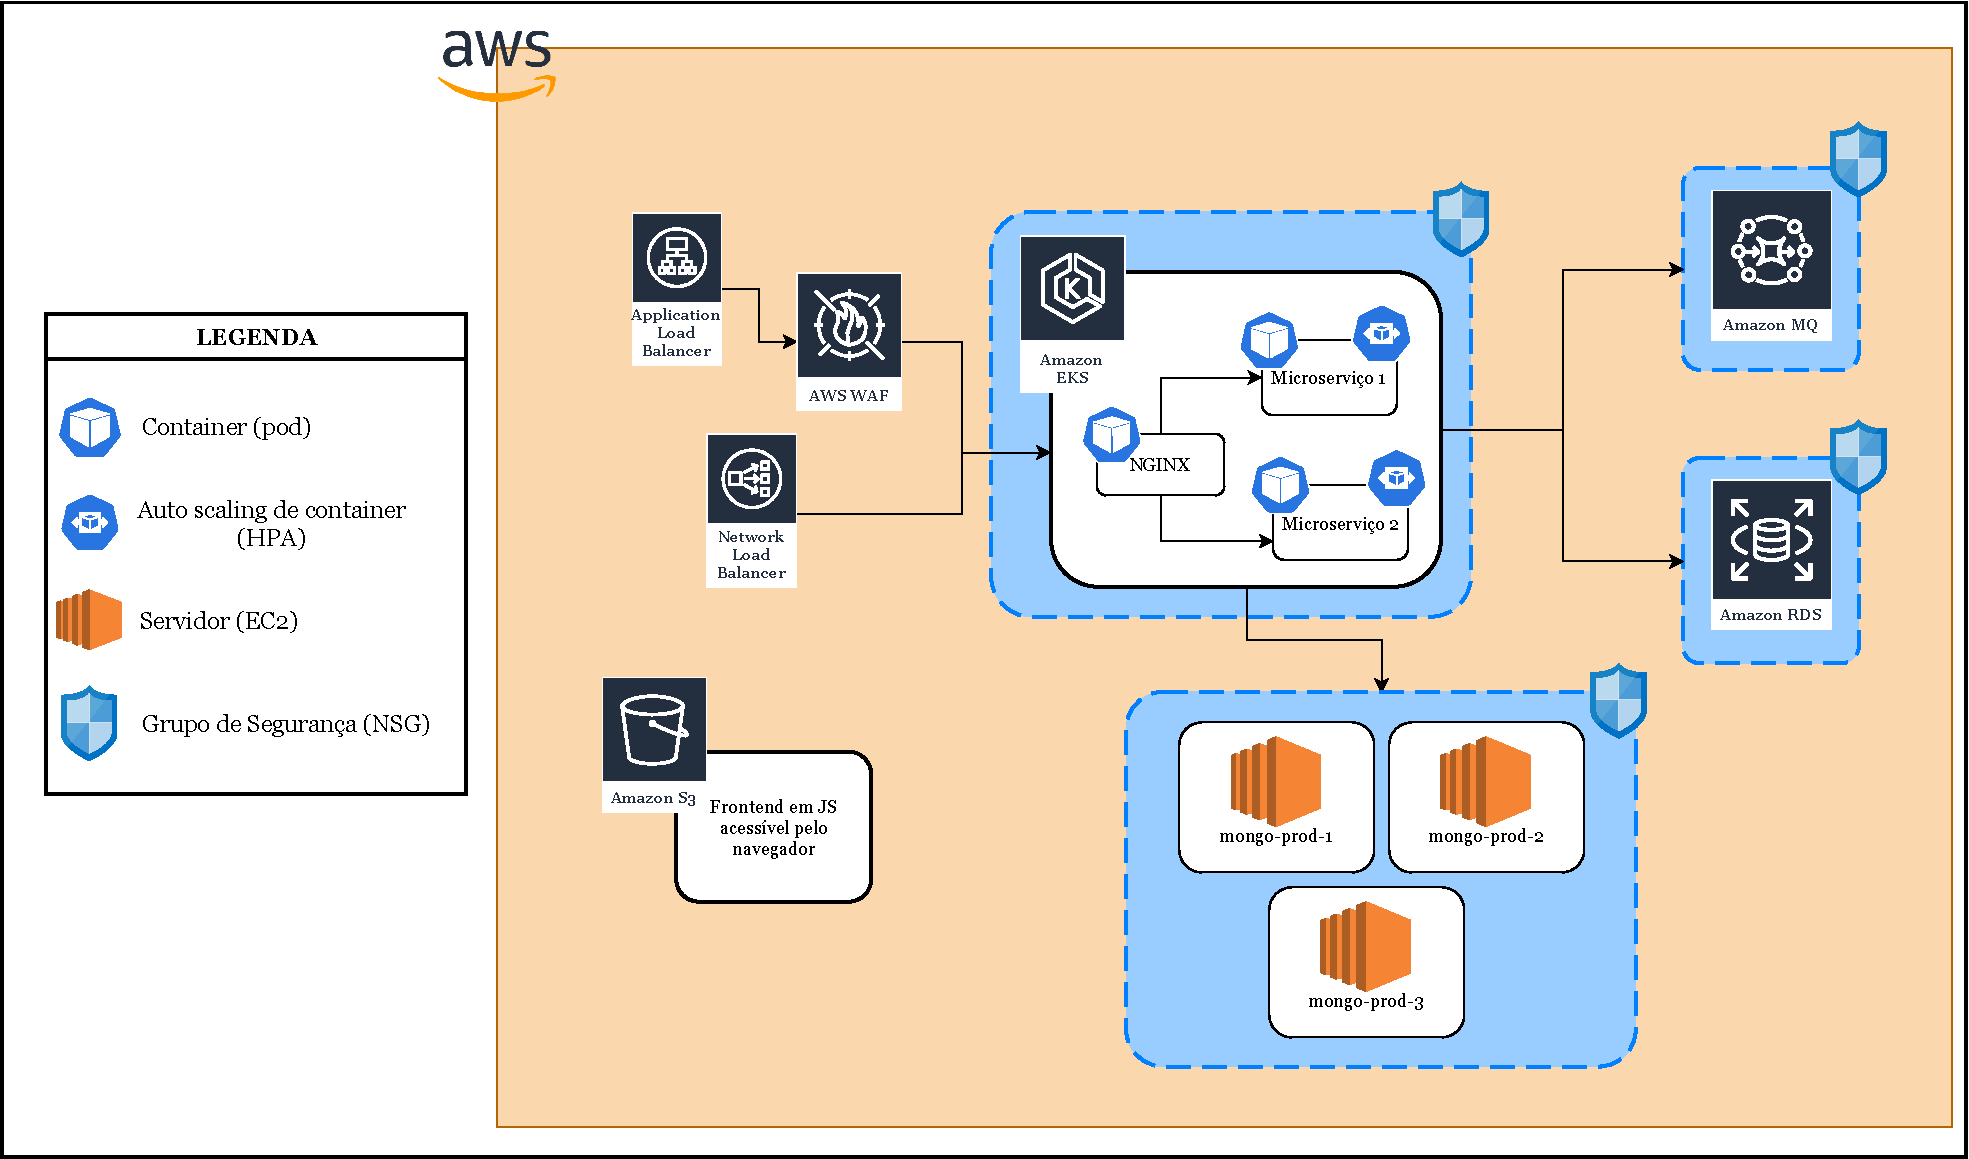
\includegraphics[width=1\textwidth]{img/diagrama.pdf}
        \end{figure}

    \section{Decisões}
        Irei falar sobre cada item primeiro, e também outras possíveis formas de solucionar.
        Depois irei comentar sobre as considerações.
        \begin{itemize}
            \item \textbf{Frontend em JS}: escolhi utilizar o s3, por ser menos uma coisa para se gerenciar manualmente. Outra opção é criar uma imagem docker deste serviço em JS para hospedar em um container no EKS, por exemplo.
            \item \textbf{Backend em microserviços}: para hospedá-los, optei pelo Kubernetes, mais especificamente o EKS (kubernetes gerenciado da AWS). Com ele é possivel hospedar vários microserviços e ter um ambiente escalável. Coloquei também o Network Load Balancer para acessar internamente e o Application Load Balancer para acessar externamente, e, também, um WAF, caso esses microserviços transitem dados sensíveis (cartão de crédito, etc., devido ao PCI).
            \item \textbf{Sistema de Mensageria}: decidi usar o RabbitMQ, pois é o que tenho mais experiência. Porém, é possível utilizar outro, como o Kafka. Optei, novamente, usar o serviço gerenciado da AWS, que é o Amazon MQ. Com ele consigo criar um cluster de RabbitMQ gerenciado, portanto, não precisamos gerenciar os servidores após criado.
            \item \textbf{Banco de dados}: Como banco SQL, escolhi o PostgreSQL, utilizando o banco de dados como serviço da AWS (RDS). E como banco não relacional, escolhi o mongo, porém, há várias outras opções, como o couchbase, redis, etc.
            \item \textbf{Carga de trabalho variada}: Isso pode ser atingido configurando o auto scaling de nós do Kubernetes (Cluster AutoScaler) e, também, utilizando o auto scaling de containers (Horizontal Pod Autoscaling). Os dois trabalham em conjunto: o autoscaling de containers irá subir um novo container conforme uma métrica (CPU), e, caso esse container não pode ser alocado em algum nó já existente, o Cluster AutoScaler irá subir um novo para que esse novo container possa ser iniciado.
        \end{itemize}

    \section{Considerações}
        \begin{itemize}
            \item \textbf{Custo baixo}: Visando o baixo custo, devemos configurar o auto scaling corretamente, para não escalar nós quando não deveria, pois isso significa mais um servidor com bastante recurso sendo sub utilizado.
            \item \textbf{Minimizar trabalho operacional}: Devido à este ponto, escolhi usar os serviços gerenciados que a AWS oferece. Dessa forma, não perdemos tempo subindo e configurando os cluster e até mesmo evitamos possíveis problemas que teríamos caso algum problema ocorresse nesses serviços.
            \item \textbf{Boas práticas}: Aqui entra o uso efetivo de todos os serviços, em especial os auto scalings. Mais uma vez cito a importância de configurar a escabilidade horizontal e vertical.
            \item \textbf{Fundamentos de rede}: Utilização de boas práticas de rede usando a AWS. Configurando corretamente as regras de firewall (nos grupos de segurança); deixando comunicar o máximo possível sem expor à internet, caso isso não seja possível, colocar um WAF para acessá-los.
        \end{itemize}

    \section{Observações Finais}
        Já criei um ambiente com os requisitos quase iguais a esse e utilizei as mesmas ferramentas. Também tive que deixar "mais seguro" por se tratar de um ambiente que era frequentemente auditado pelo PCI.
        Para este desafio, também criei um código básico em terraform para subir o ambiente na AWS, o código está aqui: \href{https://github.com/Valeyard1/desafio-devops-picpay}{https://github.com/Valeyard1/desafio-devops-picpay}.
        \newline
        \newline
        Muito obrigado.

\end{document}

